\section{Results}
\subsection{A quadratic problem}
To see how the gradient descent method works in real time, several examples will be discussed. First the function $f$ previously presented in \ref{eq:10} will be considered. As can be seen in figure \ref{fig:Merged}, $f$ attains a global minimum at $x = (0,0).$ Thus, $f$ is clearly convex. In order to verify the convexity of $f$ algebraically, lemma \ref{second-ord-cond} will be used. The partial derivatives of $f$ compute to: $f_{11}(x) = 1$, $f_{22}(x) = 10$ and $f_{12}(x) = 0$, so its Hessian is given by: $
\mathcal{H} = 
\begin{bmatrix}
1 & 0 \\
0 & 10 
\end{bmatrix}
$.
Fix $x \in \mathbf{R}^{n} = \textbf{dom} (f).$ Then $x^{T} \mathcal{H} x = (x_{1}, x_{2}) \mathcal{H}  
\begin{pmatrix}
    x_{1} \\
    x_{2} 
\end{pmatrix}
= x_{1}^{2} + 10x_{2}^{2} \geq 0.
$
Since $x$ was arbitrarily fixed, the inequality holds $\forall x \in \mathbf{R}^{n} = \textbf{dom} (f).$ Therefore, $\mathcal{H}$ is positive semidefinite. Then by the lemma \ref{second-ord-cond}, the function $f$ is convex.
\subsubsection{Gradient descent with fixed step size}
The first observation is that $f$ is $\alpha$-strongly convex with $\alpha=1$, since $\mathcal{H} - I = \begin{bmatrix}
0 & 0 \\
0 & 9
\end{bmatrix}$ is positive semidefinite. This holds by theorem \ref{SPD_e}, as all the eigenvalues of $\mathcal{H} - I$ are non-negative. Also, $\mathcal{H}^{T}\mathcal{H} = \mathcal{H}^{2}= \begin{bmatrix}
1 & 0 \\
0 & 100
\end{bmatrix}$.
The spectral norm of $\mathcal{H}$ is $\vertiii{\mathcal{H}}_{2} = \sqrt{100} = 10.$ Then by remark \ref{findL} $f$ has Lipschitz continuous gradient with $L=10.$ By the results obtained from the convergence analysis of gradient descent, choosing the step size $\tau$ such that $\tau \leq \max\{2\alpha / L^{2},\text{ } 2/(\alpha+L)\} = \max\{1/50,\text{ } 2/11\} = 2/11$ ensures convergence. The starting point is chosen to be $x^{(0)}=(10,2)$ and the stopping criterion $\eta = 10^{-7}.$ The situation will be analyzed for values of $\tau \in \{\frac{2}{11}, \frac{1}{11}, \frac{1}{22}, \frac{1}{44}\}.$ The algorithm will compute a minimizing sequence consisting of $N$ vectors. Including the starting point, this sequence will be: $(x^{(0)},\ldots,x^{(N)}).$ The function value of $f$ evaluated at these vectors decreases iteration after iteration and gets closer and closer to the exact global minimum. For each $\tau,$ the value of interest is $N$, which denotes the total number of iterations until the the algorithm terminates. This happens, once the stopping criterion is reached, i.e.,  $||\nabla f(x)||_{2} \leq \eta$. It is important to realize that in this particular problem, the exact global minimum $p^{*}$ is known, namely when $x^{*}=(0,0),\text{ } p^{*} = f(x^{*}) = 0$. The optimality gap is the distance between the function value at the final iterate $f(x^{(N)})$ and $p^{*} = 0$ which is precisely $f(x^{(N)}).$  The convergence with the fixed step size can be visualized. The figure below shows the convergence to the optimal solution $p^{*}$ as the number of iterations $k$ increases, using different step sizes $\tau$.\footnote{See line~\ref{line:13} to~\ref{line:14} for the code to create the plots.}
\begin{figure}[h!]
    \centering
        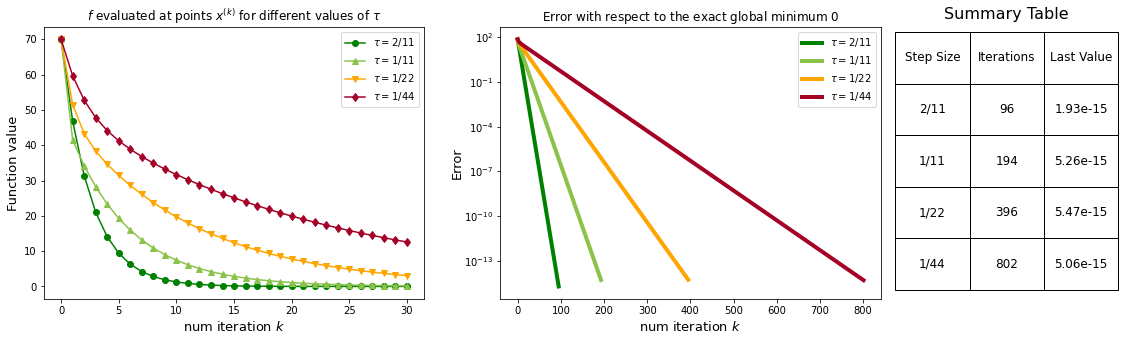
\includegraphics[width=1\textwidth]{Pictures/Merged_conv_ellipsoid_fixed_table.png}
    \caption{The left plot illustrates the convergence, while the middle plot shows the logarithmic error $f(x^{(k)})$ at each iteration up to the final iteration. On the right, a table summarizes the step sizes used, the total number of iterations, and the optimality gap.}\label{fig:convergence1_fixed}
\end{figure}\\
In order to visualize the convergence more effectively, contour plots can be very useful. A contour plot is a type of graph that shows how a function of two variables changes across different values. It does this by plotting contour lines, which are lines that connect points with the same value of the function. These contour lines help us visualize how the value of the function changes as we move around the graph. This can be particularly helpful for seeing how the gradient descent algorithm is moving towards the global minimum.
\newpage
The convergence can be visualized for different step sizes $\tau$. Let's choose $\tau_1 = 1/51$ and $\tau_2 = 2/11$. For step size $\tau_1$, gradient descent computes a minimizing sequence consisting of 930 vectors, and for $\tau_2$, as can be seen in the summary table in Figure \ref{fig:convergence1_fixed}, it computes a minimizing sequence consisting of 96 vectors. The contour plot below demonstrates the convergence for both step sizes by plotting the starting point $x^{(0)}=(10, 2),$ the two minimizing sequences and the contour lines of $f.$\footnote{See line~\ref{line:15} to~\ref{line:16} for the code to create the contour plot.}
\begin{figure}[h!]
    \centering
        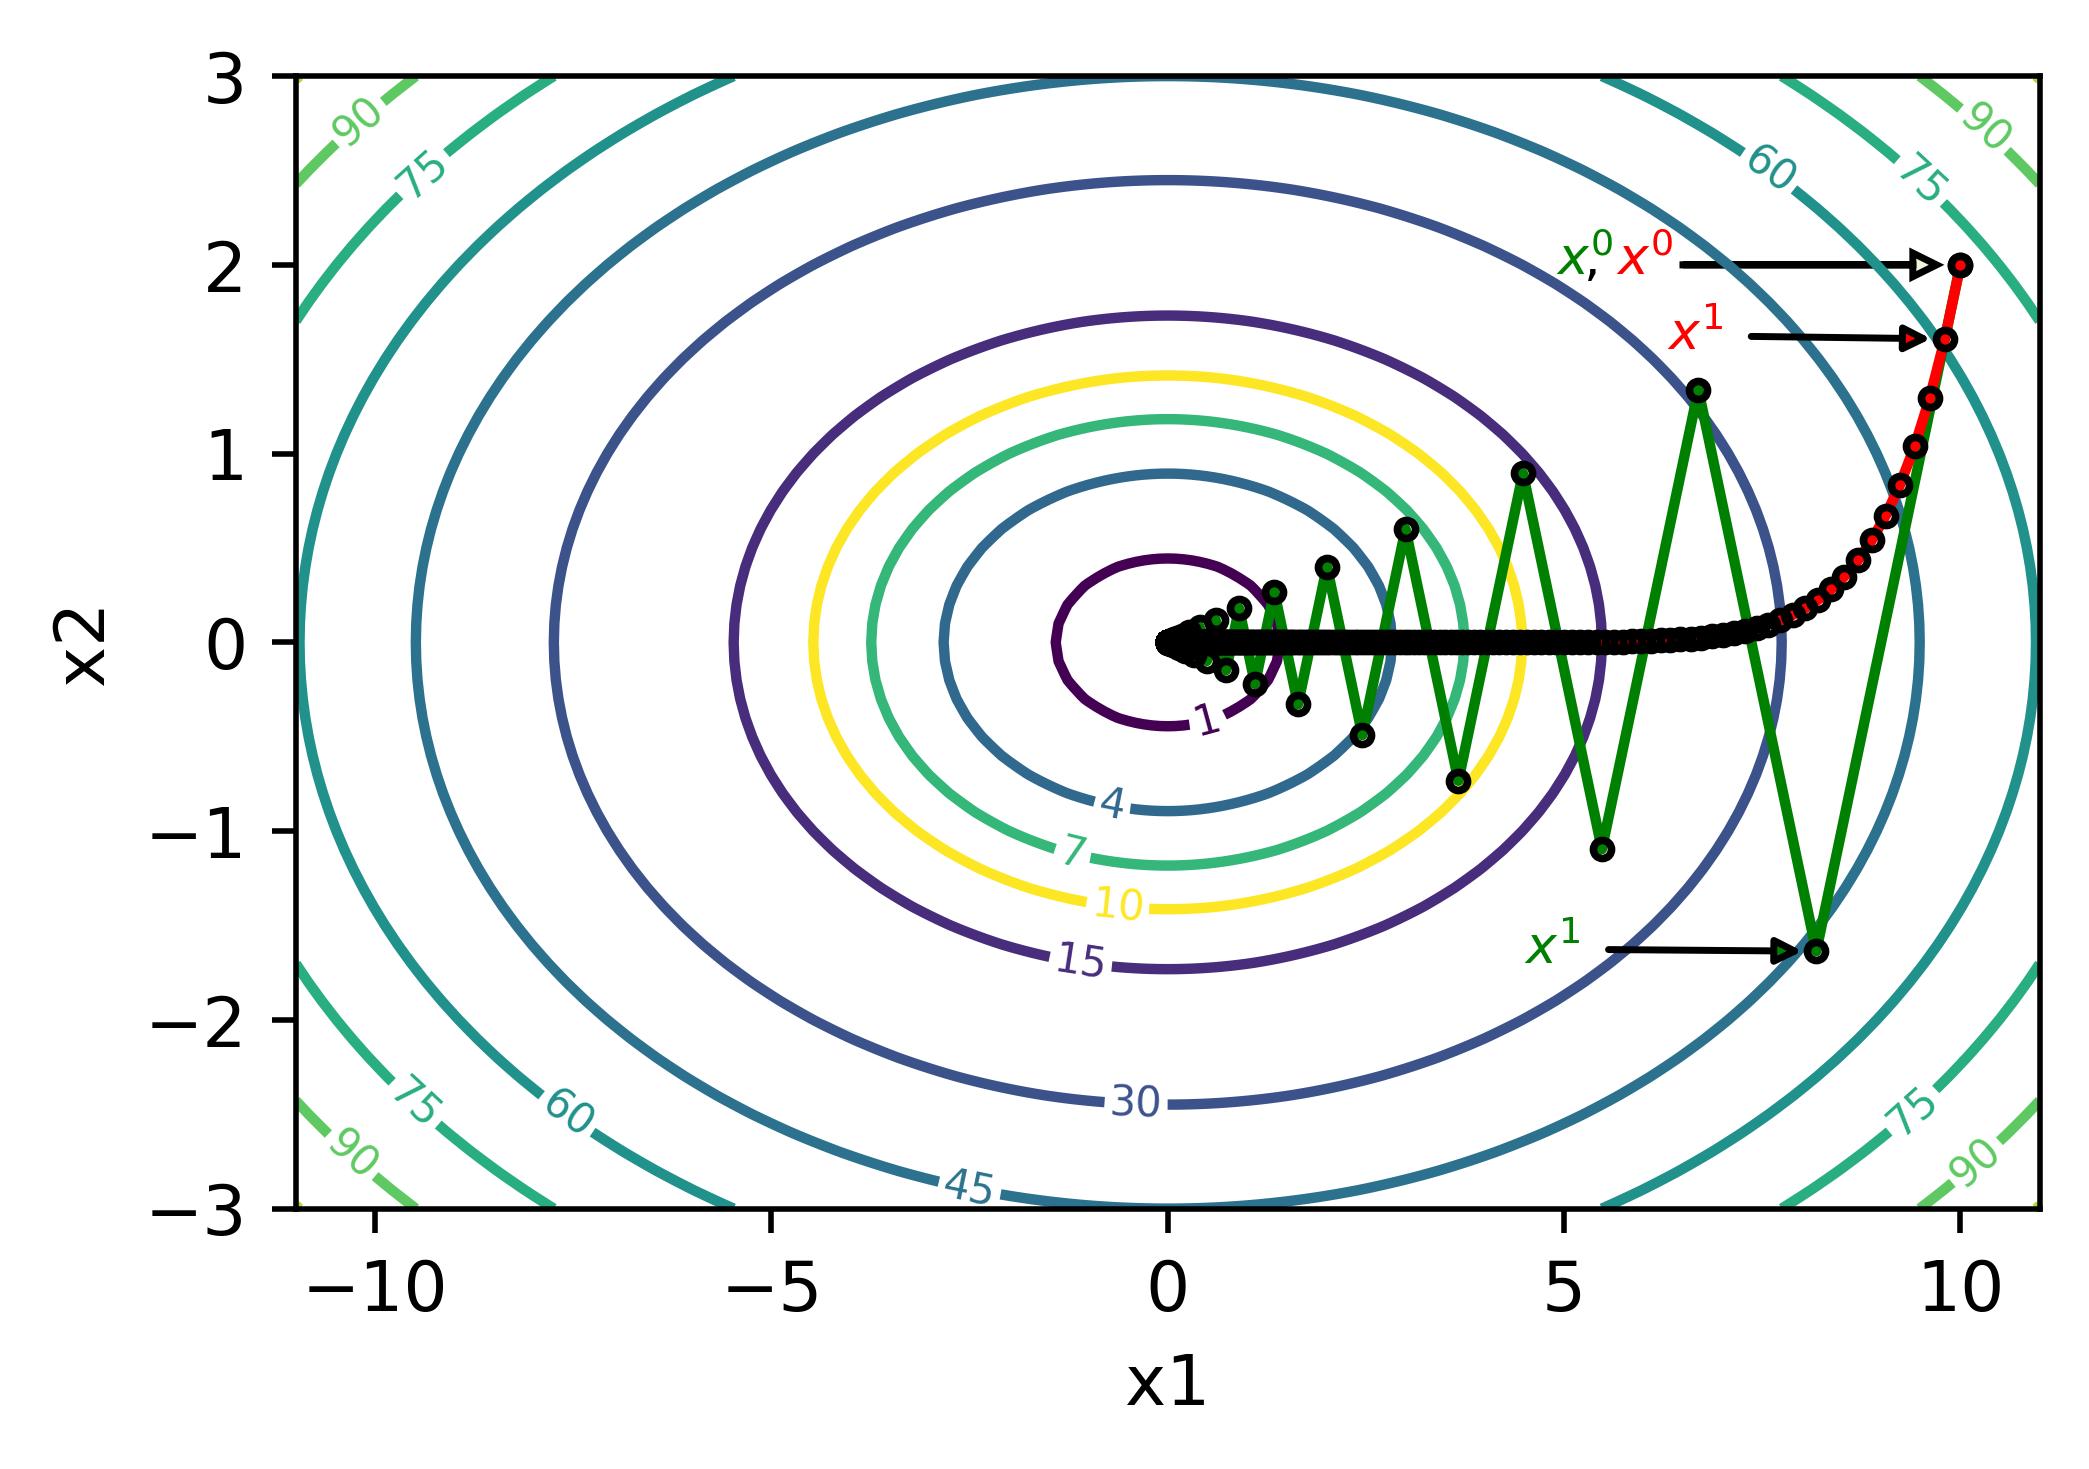
\includegraphics[width=0.65\textwidth]{Pictures/Level sets of ellipsoid_fixed.png}
    \caption{The color red represents the convergence with step size $\tau_{1}$ and green represents the convergence with step size $\tau_{2}.$ With step size $\tau_{2}$, the convergence is substantially faster than with step size $\tau_{1}.$ For sake of illustration $\tau_{1}$ was chosen to be compared to $\tau_{2}$, since $\tau_{1}$ satisfies the bound provided by \ref{pf_gd_sc_L}.}\label{fig:levelsets1_fixed}
\end{figure}\\
It is important to note that choosing a bound larger than $\tau_{2} = 2/11$ can cause some problems. In fact you can find yourself in unknown territory. Since if both $\tau \leq 2/(\alpha + L) $ and $\tau < 2\alpha / L^{2}$ are ignored, the likelihood that the algorithm diverges or overshoots the minimum, increases. The figure below shows the relation between the number of iterations until the algorithm terminates and the step size.\footnote{See line~\ref{line:17} to~\ref{line:18} for the code to create the plot.} 
\begin{figure}[h!]
    \centering
        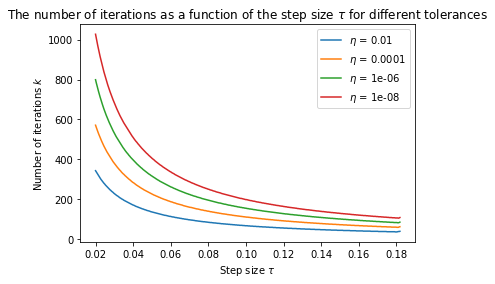
\includegraphics[width=0.75\textwidth]{Pictures/GD ellipsoid_fixed_iterations_vs_stepsize.png}
    \caption{As long as $\tau$ remains within the appropriate range, an increase in $\tau$ leads to faster convergence towards the global minimum, and hence a reduction in the number of iterations required for termination. Additionally, an increase in the tolerance $\eta$ results in faster convergence.}\label{fig:GD_ell_fixed_iter}
\end{figure}\\
\newpage
\subsubsection{Gradient descent with backtracking line search} Gradient descent using backtracking line search with $\alpha = 0.3$, $\beta = 0.8$ and $\eta = 10^{-7}$ is implemented on the quadratic function $f$.\footnote{See subsection \ref{GD-on-qd} for the implementation of GD with backtracking line search on $f.$} The number of iterations until the algorithm terminates is 92. So the algorithm computes a minimizing sequence that consists of 93 vectors: $(x^{(0)},\ldots,x^{(92)})$. The convergence of gradient descent to the exact global minimum $p^{*}=0$ with backtracking line search, can be visualized.\footnote{See line~\ref{line:p5} to~\ref{line:p6} for the code to create the convergence plots.} The optimality gap is the distance between $f(x^{(92)}) = 3.5\cdot 10^{-15}$ and $p^{*}=0$ which is precisely $f(x^{(92)}).$ In the following figure, on the left you can see an illustration of the convergence to $p^{*}=0$ and on the right the error $f(x^{(k)})$ with respect to $p^{*}=0$ for every $k$ up until 30.
\begin{figure}[h!]
    \centering
        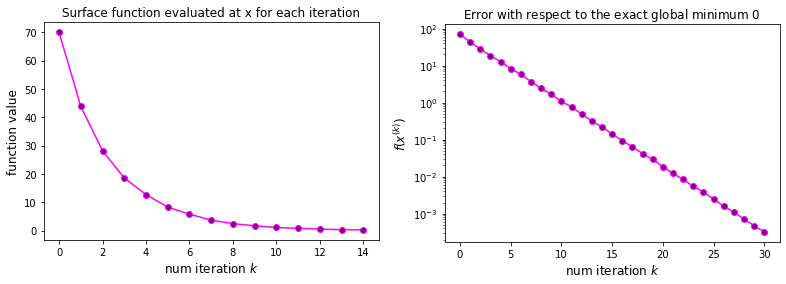
\includegraphics[width=0.85\textwidth]{Pictures/Merged_conv_ellipsoid.png}
    \label{fig:convergence1}
\end{figure}\\
The contour lines of the quadratic function $f$ and the points $(x^{(0)},\ldots,x^{(92)})$ are shown in the figure below.\footnote{See line~\ref{line:p7} to~\ref{line:p8} for the code to create the contour plot.}
\begin{figure}[h!]
    \centering
        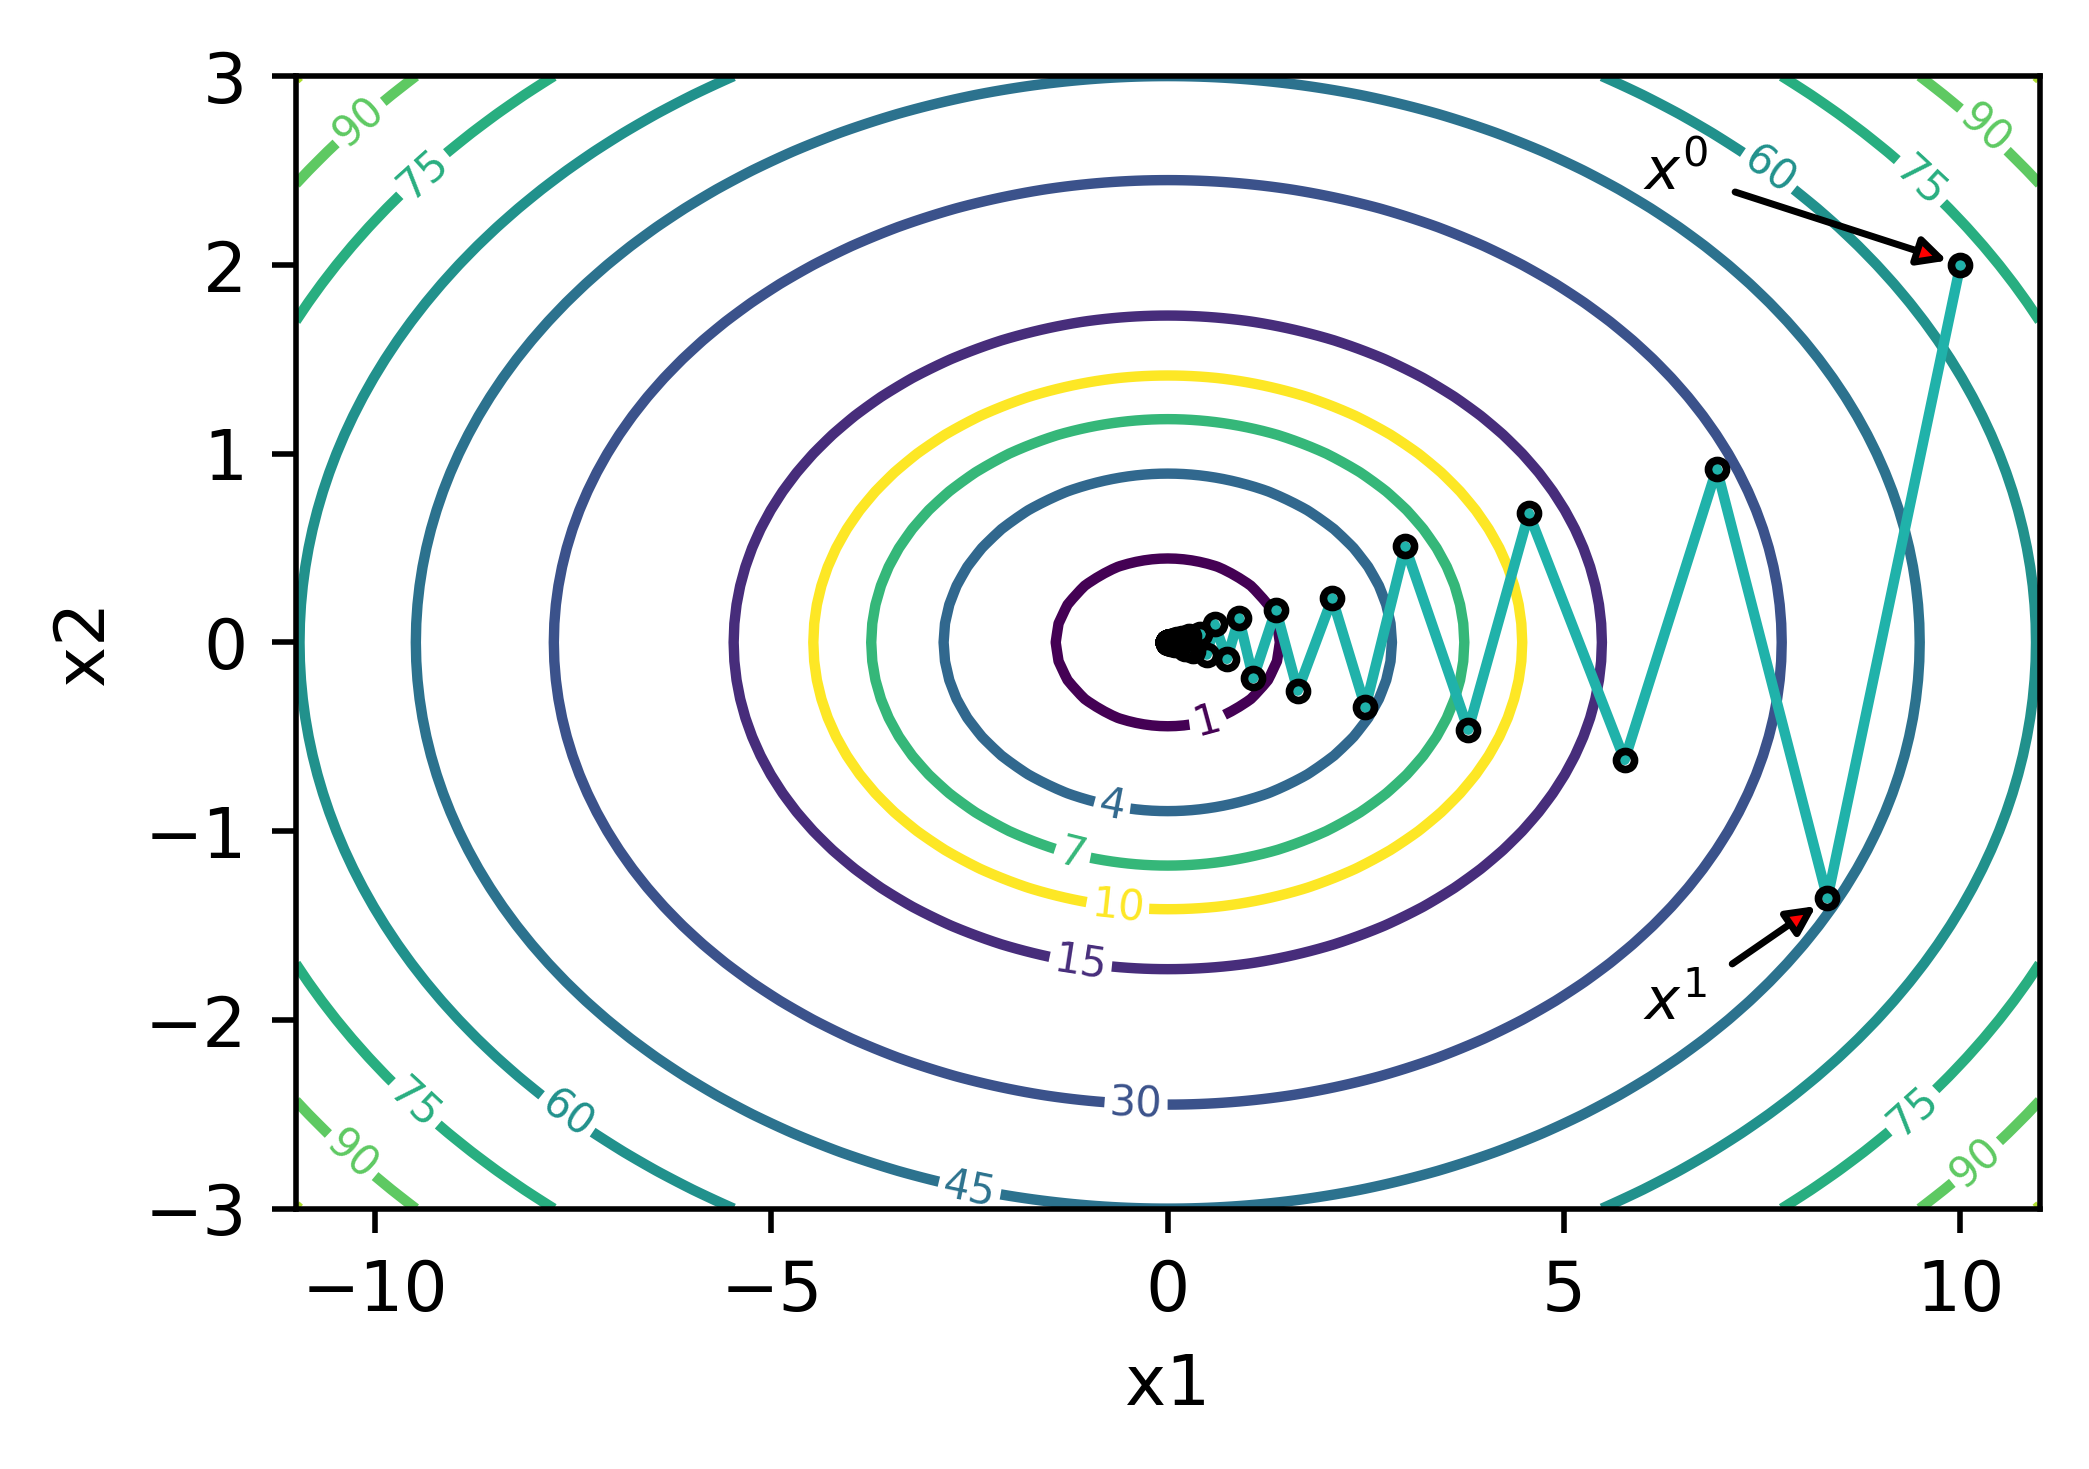
\includegraphics[width=0.58\textwidth]{Pictures/Level sets of ellipsoid.png}
    \label{fig:levelsets1}
\end{figure}
\newpage
\subsection{A non-quadratic problem}
We now consider a non-quadratic example in $\mathbf{R}^2$,  with 
\begin{equation*}\label{eq:12}\tag{5.2.1}
\begin{aligned}  
    &g(x) = e^{x_{1}+3x_{2}-0.1}+e^{x_{1}-3x_{2}-0.1}+e^{-x_{1}-0.1}
\end{aligned}
\end{equation*}
First it should be checked whether this function is convex. $g(x) = g_{1}(x)  + g_{2}(x) + g_{3}(x).$ Define: $f: y \mapsto e^{y}$. Then $g_{i}(x) = f(h_{i}(x)) \text{ } i=1,2,3$ and $g(x) = f(h_{1}(x)) + f(h_{2}(x)) + f(h_{3}(x)) ,$ where $h_{1}: x \mapsto x_{1} + 3x_{2}-0.1$, $h_{2}: x \mapsto x_{1} - 3x_{2}-0.1$, and $h_{3}: x \mapsto -x_{1}-0.1$. Since $f"(y) = e^{y} > 0 \text{ }$ for all $y \in \mathbf{R},$ $f$ is convex. Furthermore $h_{1}, h_{2}, h_{3}$ are affine. By definition \ref{compaf} the composition of a convex function with an affine function is convex, so $g_{i}(x) = f(h_{i}(x))$ is convex for $i=1,2,3.$ The sum of convex functions is also convex, therefore $g$ is convex. To get a visual impression, figure \ref{fig:exp} is a 3D plot of $g.$
\begin{figure}[h!]
    \centering
        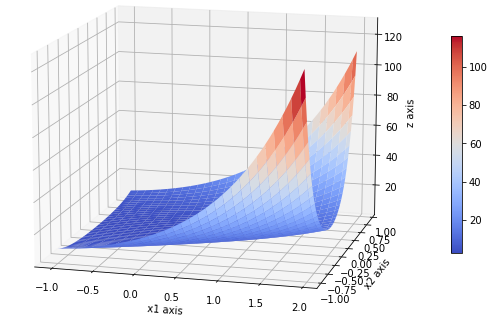
\includegraphics[width=0.36\textwidth]{Pictures/3D plot of an exponential function.png}
    \caption{3D surface plot of the function $g$}\label{fig:exp}
\end{figure}\\
Gradient descent using backtracking line search with $\alpha = 0.1$, $\beta = 0.7$ and stopping criterion $\eta = 10^{-7}.$ is implemented on the non-quadratic function $g$.\footnote{See subsection \ref{GD-on-nqd} for implementation of GD with backtracking line search on $g$.} The starting vector is chosen to be $x^{(0)} = (-1,0.5)$. The algorithm computes a minimizing sequence of 39 vectors. Together with the starting point we find the sequence: $(x^{(0)},\ldots,x^{(39)}).$ The function value decreases iteration after iteration and whenever $||\nabla f(x)||_{2} \leq \eta$, the algorithm terminates. The figure below shows the convergence to the global minimum $p^{*} \approx g(x^{(39)})=2.559$, where the plot on the left is an illustration of the convergence to $p^{*}$ and the one on the right the error $g(x^{(k)}) - g(x^{(39)})$ for every k up until 39.\footnote{See line~\ref{line:p9} to~\ref{line:p10} for the code to create the convergence plots.} 
\begin{figure}[h!]
    \centering
        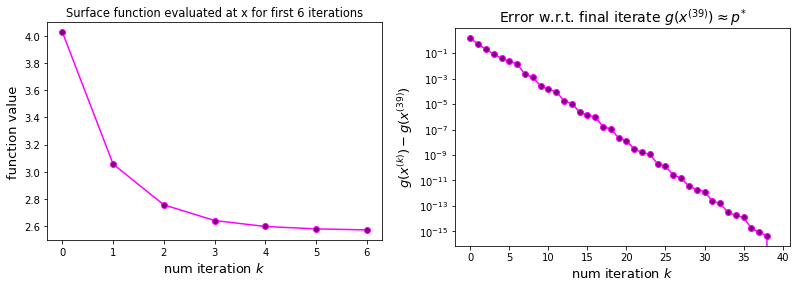
\includegraphics[width=0.72\textwidth]{Pictures/Merged_conv_exponential.png}
    \label{fig:convergence2}
\end{figure}\\
Similarly to the the quadratic function, it is possible to provide a contour plot for $g.$ The contour lines of the non-quadratic function $g$ and the points $(x^{(0)},\ldots,x^{(39)})$ are shown in the figure below.\footnote{See line~\ref{line:p11} to~\ref{line:p12} for the code to create the contour plot.}
\begin{figure}[h!]
    \centering
        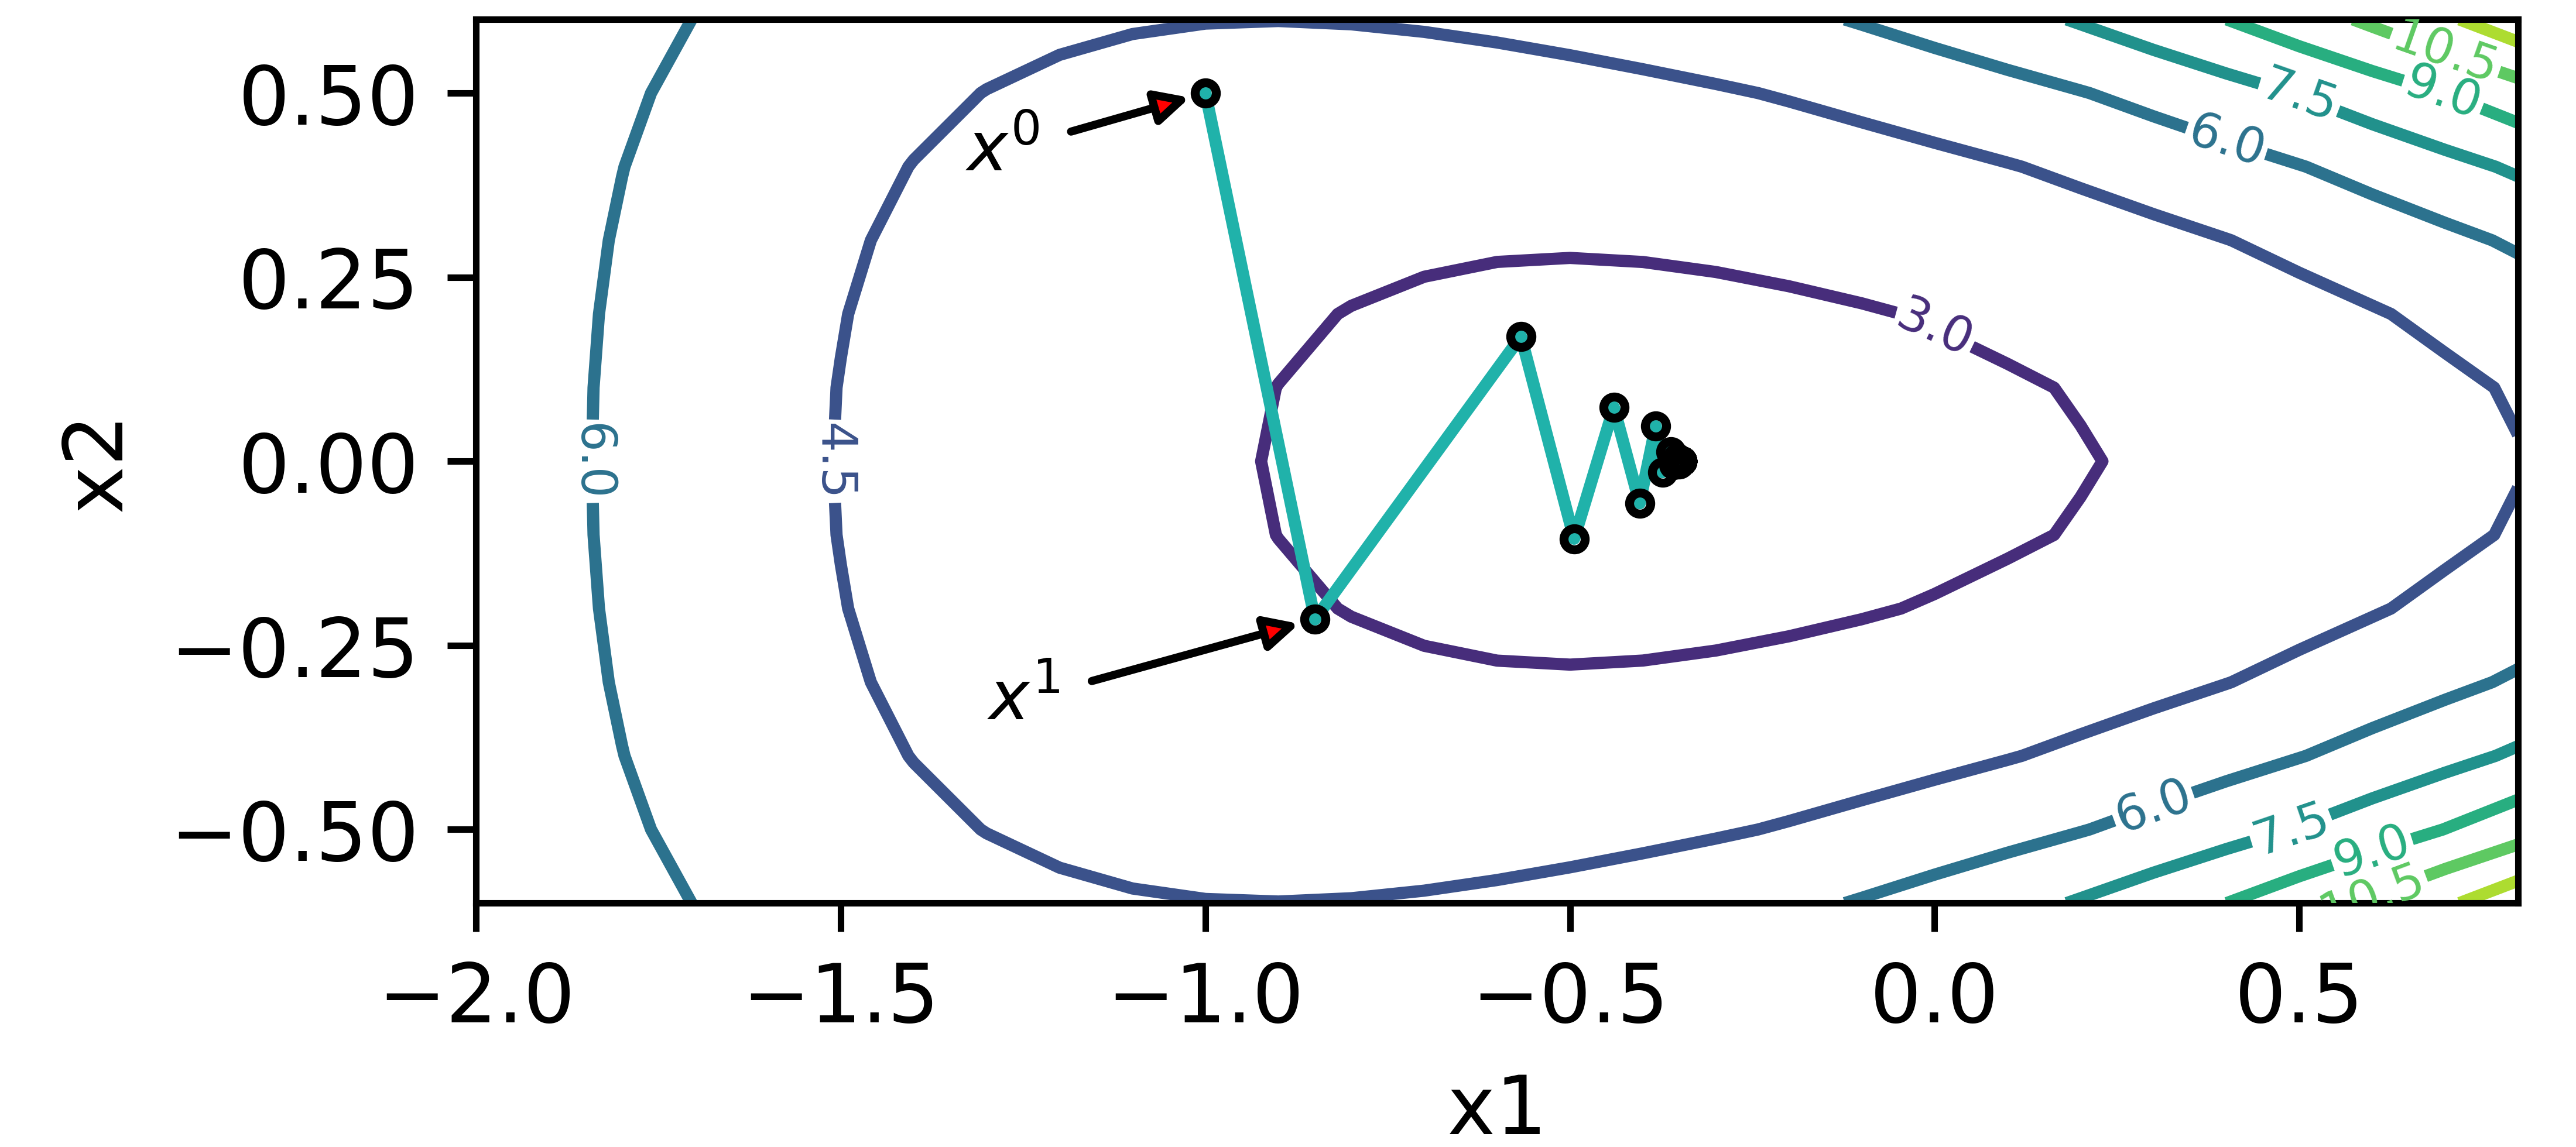
\includegraphics[width=0.55\textwidth]{Pictures/Level sets of exponential.png}
    \label{fig:levelsets2}
\end{figure}\\
\newpage
\subsection{A multi-dimensional non-convex problem}
The function that will be considered is Ackley's function.\ref{eq:18} This function is widely used for testing optimization algorithms.\cite{Test_functions} In its two-dimensional form, as shown in \ref{fig:Ackelys_plot}, it is characterized by a nearly flat outer region, and a large hole at the centre.\footnote{See line~\ref{line:19} to~\ref{line:20} for the code to create 3D plots of Ackley's function.}
\begin{equation*}\label{eq:18}\tag{5.3.1}
\begin{aligned}
&h(x) = -a\exp\left(-b\sqrt{\frac{1}{d}\sum_{i=1}^{d} x_{i}^{2}}\right) - \exp\left(\frac{1}{d}\sum_{i=1}^{d} \cos(cx_{i})\right) + a + \exp(1) 
\end{aligned}
\end{equation*}
\begin{figure}[h!]
    \centering
        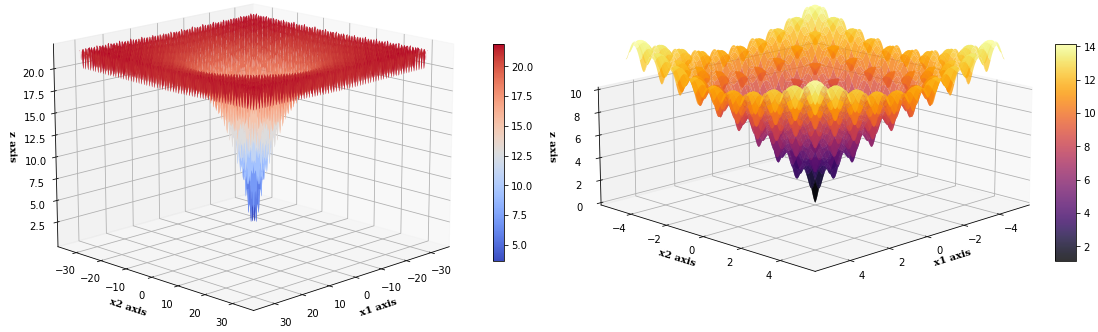
\includegraphics[width=0.85\textwidth]{Pictures/Merged_Ackleys_plot.png}
    \caption{3D plots of $h$ on $x_{i} \in [-32.768,\text{ } 32.768]$, and on $x_{i} \in [-5,\text{ } 5]$}\label{fig:Ackelys_plot}
\end{figure}\\
 Many loss functions in machine learning are non-convex. $h$ is an example of a non-convex function that is multimodal, i.e., it has multiple local minima. This possesses a risk for gradient-based optimization methods, since they can become trapped in one of the local minima and thus fail to find the global minimum. Therefore, it is a good benchmark function to evaluate the performance of gradient-based optimization methods. The global minimum of $h$ is known, namely when $x^{*} = \vec{0}$ , $h(x^{*}) = 0.$ 
 \subsubsection{Gradient descent with backtracking line search}
 Consider $h$ with dimension $d=100.$ For the variable values take: $a = 20,\text{ }b = 0.2,$ and $c = 2\pi$. Gradient descent using backtracking line search with $\alpha = 0.1, \beta = 0.8$ and stopping criterion $\eta = 1e-6$ is implemented on $h.$\footnote{See subsection \ref{GD-Ack} for implementation of GD with backtracking line search on $h.$} To test convergence, a vector $x^{(0)}$ is created randomly such that each term lies in $[-32.768, 32.768]$.\footnote{See \ref{line:21} for the code to create a random vector.} Secondly, the algorithm is tested by choosing a starting vector that is close to the origin, namely $x^{(0)}=(0.4,\ldots,0.4).$ Figure \ref{fig:Ackelys_conv_check} shows the progression of the algorithm for the two different starting vectors.\footnote{See line~\ref{line:22} to~\ref{line:23} for the code to create the convergence plots.}
\begin{figure}[h!]
    \centering
        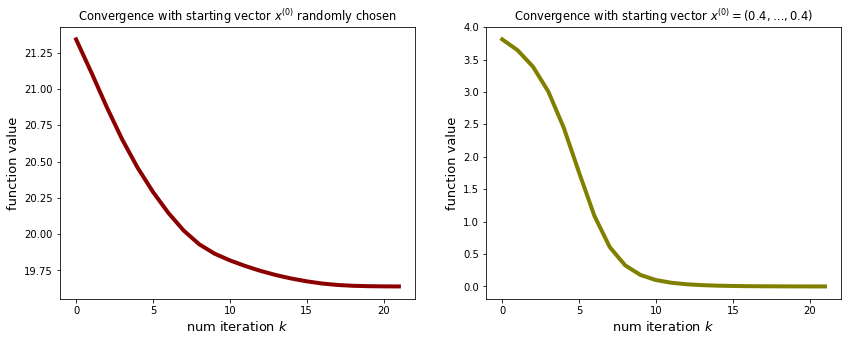
\includegraphics[width=0.75\textwidth]{Pictures/Merged_conv_ackleys.png}
    \caption{Plots to check convergence of GD for two different starting vectors.}\label{fig:Ackelys_conv_check}
\end{figure}\\
\newpage
From the results in Figure \ref{fig:Ackelys_conv_check}, the main limitation of gradient descent becomes evident: it is highly susceptible to local minima due to its inherent reliance on gradient information. For a randomly created starting vector, the algorithm converges towards one of the many local minima of $h$, and only if $x^{0}$ is chosen to be very close to the optimal solution, it achieves convergence towards the global minimum. This experiment underscores the importance of selecting appropriate optimization methods for specific problems. A natural question that arises is whether stochastic gradient descent (SGD) can be applied to this problem. SGD is specifically designed for objective functions that arise in machine learning and deep learning, which typically involve large datasets. However, $h$ is a mathematical optimization problem that does not have the desirable form of a sum of functions. Consequently, there is no natural way to divide the function into smaller subsets. In other words, the gradient information in $h$ is deterministic and does not depend on a dataset, which eliminates stochasticity from the problem and makes SGD less applicable.

\subsubsection{Simulated Annealing}
An alternative to gradient descent is simulated annealing with pseudo-code given in \ref{Pseudocode_SA}. The problem parameters remain unchanged: $d=100, a=20, b=0.2,$ and $c=2\pi.$ The algorithm is tested for two different starting vectors, namely one that is randomly generated with terms lying in $\left[-32.768,32.768\right]$ and one that is closer to the optimal solution with terms in $\left[-5,5\right].$ The initial temperature is chosen to be $t_0=5.0$ and cooling schedule $t_{k} = 0.99^{k}t_0.$ The algorithm terminates when the maximum number of iterations $k_{max}=400$ is reached. The figures \ref{fig:SA_conv1} and \ref{fig:SA_conv2} below depict the possible paths the algorithm can take to progress towards the global minimum of $h$. In the left figure, the algorithm converges for both starting vectors, whereas the right figure shows a scenario in which the algorithm for one of the starting vectors gets trapped in a local minimum of $h$. 

\begin{figure}[h]
  \centering
  \begin{minipage}[b]{0.3687\textwidth}
    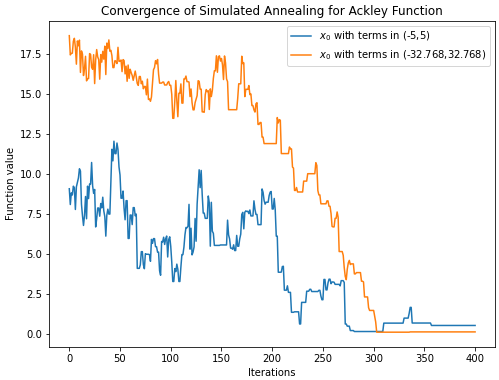
\includegraphics[width=\textwidth]{Pictures/sa_convergence-ackley3-38-c.png}
    \caption{Example 1}\label{fig:SA_conv1}
  \end{minipage}
  \hspace{0.05cm} 
  \begin{minipage}[b]{0.36\textwidth}
    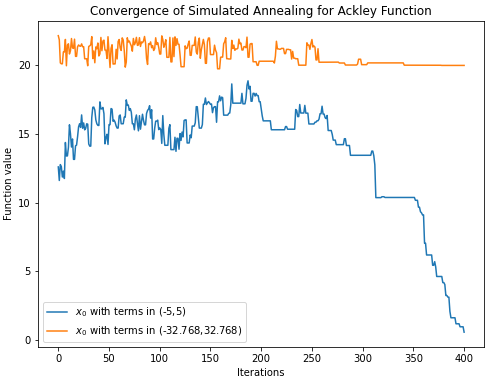
\includegraphics[width=\textwidth]{Pictures/sa_convergence-ackley3-37_c.png}
    \caption{Example 2}\label{fig:SA_conv2}
  \end{minipage}
\end{figure}
In order to visualize the stochasticity in the algorithm, $h$ with dimension $d=2$ is considered. In this setting, contour plots of $h$ and the progression of simulated annealing towards possibly the global minimum can be plotted. The figures \ref{fig:SA_cont1} and \ref{fig:SA_cont2} below depict the progression of two different starting vectors in $\mathbf{R}^2$ with terms in $\left[-10, 10\right]$ towards the global minimum.
\begin{figure}[h]
    \centering
    \begin{minipage}[b][0.38\textwidth]{0.35\textwidth}
      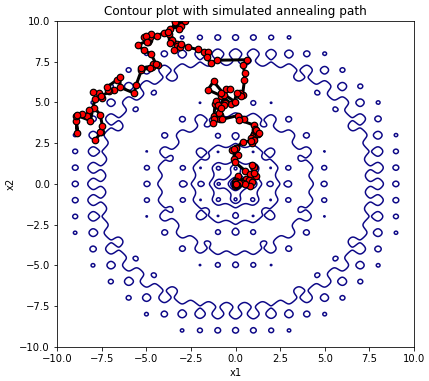
\includegraphics[width=\textwidth]{Pictures/sa_convergence-ackley_contour11.png}
      \caption{Example 1}\label{fig:SA_cont1}
    \end{minipage}
    \hspace{0.05cm}
    \begin{minipage}[b][0.38\textwidth]{0.35\textwidth}
      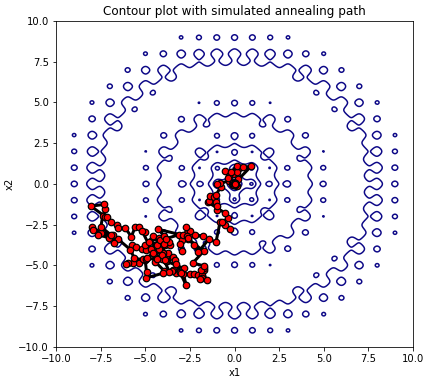
\includegraphics[width=\textwidth]{Pictures/sa_convergence-ackley_contour18.png}
      \caption{Example 2}\label{fig:SA_cont2}
    \end{minipage}
\end{figure}
\subsubsection{Particle Swarm Optimization (PSO)}
As described in Section \ref{PSO_s}, Particle Swarm Optimization (PSO) is a stochastic global optimization algorithm that performs well on multi-dimensional non-convex functions. As such, it is worth applying to minimize $h$. The algorithm is implemented in Python with cognitive and social constants set to $C_{1}=0.5$ and $C_{2}=0.3$, respectively, and the maximum number of iterations is set to $k_{max}=2000$. The only remaining parameter to determine is the size of the swarm. It is insightful to visualize the trajectory of the best function evaluations (i.e., the lowest function values in each iteration) up until termination for different swarm sizes. The following figure displays the trajectories for various swarm sizes, specifically for $N=50$, $N=200$, $N=500$, and $N=1000$. The table on the right provides the best cost (lowest function evaluation) for each of the four swarm sizes. The results are presented below (Figure \ref{fig:PSOConvMultipleSwarmSizes}).
\begin{figure}[h!]
    \centering
        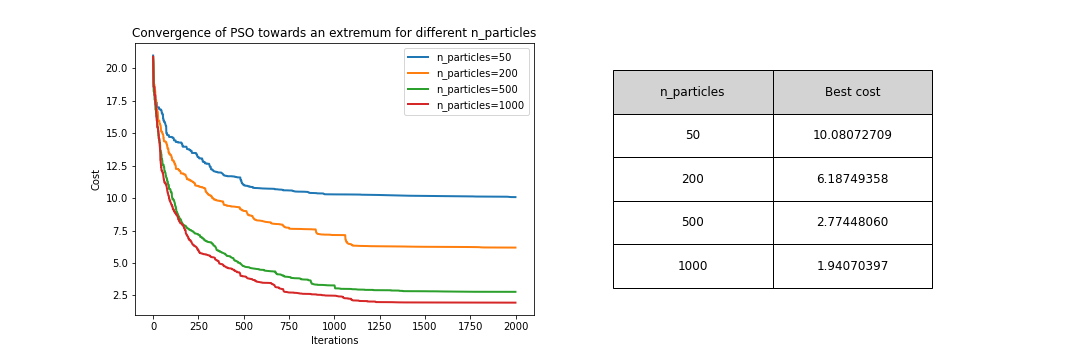
\includegraphics[width=1.12\textwidth]{Pictures/PSO_convergence-ackley_multiple_n_particles_with_table.png}
    \caption{This figure displays four trajectories of PSO distinguished by different swarm sizes n$\textunderscore$particles on the left and the best cost obtained for each of the cases in a table on the right.}\label{fig:PSOConvMultipleSwarmSizes}
\end{figure}\\
As can be seen from the figure, an increase in the swarm size, leads to convergence towards a minimum with a lower cost. It can also be noted, that none of the four cases reach the global minimum. This has to do with the design of the algorithm. PSO does not allow for worse function values (i.e., ones that are higher than the previous iterations), therefore it is sensitive to getting stuck in local minima. $h$ contains many local minima, and some of these local minima are very close to the global minimum. The number of local minima increases when the dimensionality of the problem increases. Since in this example, the dimension is $d=100,$ it becomes very unlikely for the swarm to collectively reach the global minimum. When $d$ is kept low, the likelihood that the algorithm succeeds in reaching the global minimum increases. To see whether this is indeed the case, PSO is performed on $h$ with $d=2.$ $C_{1}$ and $C_{2}$ remain unchanged. $k_{max}$ is set to $100$ and the size of the swarm is set to $50.$ The following figure shows the trajectory of the swarm towards the global minimum. Three different time steps are taken, namely $k=0,$ $k=10,$ and $k=100.$ For each time step a contour plot of the function and the positions of the particles are depicted in figure (Figure \ref{fig:PSO_2D_swarm}) below.
\begin{figure}[h!]
    \centering
        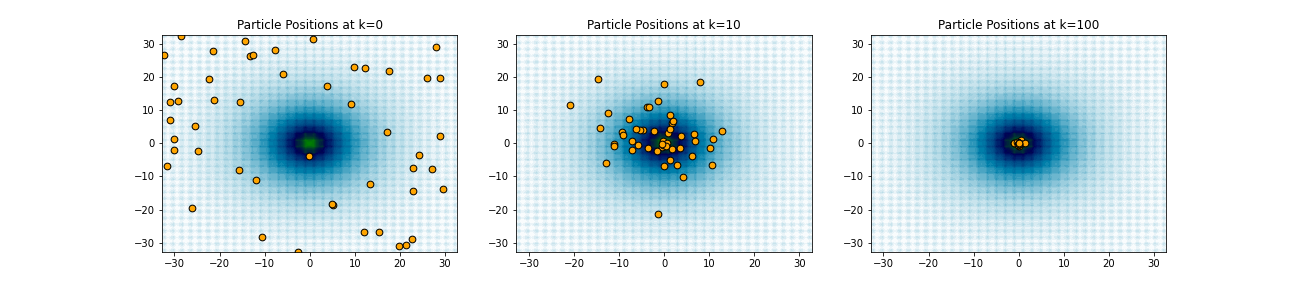
\includegraphics[width=1\textwidth]{Pictures/PSO_ackleys_2D_swarm.png}
    \caption{Contour plots and particle positions at time steps $k=0,$ $k=10,$ and $k=100$}\label{fig:PSO_2D_swarm}
\end{figure}\\
\newpage
\subsubsection{Comparison of Methods}
The effectiveness of various optimization methods was compared in minimizing Ackley's function $h$. First, gradient descent with backtracking line search was implemented. Before the implementation, it was anticipated that the algorithm's likelihood of finding the global minimum would be low. This is because Ackley's function contains numerous local minima that are closely spaced, and since gradient descent is highly sensitive to extrema, it can easily get stuck in a local minimum that isn't the global minimum. The results support this notion, as the algorithm became stuck in a local minimum when starting from a random vector. Next, simulated annealing (SA) was implemented and found to perform quite well. In fact, it was able to locate the global minimum. The primary reason for this success is that the algorithm is designed to escape local minima easily by allowing hill-climbing moves, which temporarily worsen the function evaluation outcome. Finally, particle swarm optimization (PSO) was implemented. This algorithm performed better than gradient descent by finding superior solutions, but it was still outperformed by SA, as it could not locate the global minimum. Additionally, to obtain a better solution with PSO, the swarm size had to be significantly increased, which greatly impacted computation time. In conclusion, both SA and PSO performed better than gradient descent. However, it is important to note that these algorithms were more computationally expensive, as their execution required more time than gradient descent.

\subsection{Application of SGD on a Neural Network}
\subsubsection{The Data}
In the realm of optimization, Stochastic Gradient Descent (SGD) is often applied to suitable functions associated with feed-forward neural networks. These networks are chosen because the objective functions that they generate typically take the form of a large sum of smaller functions. In each iteration of SGD, the gradient of one of these smaller functions, $\nabla f_{i(k)}(x_{k})$ where $i(k)$ is drawn uniformly at random from $\{1,\ldots,n\}$, is computed. Here, $n$ denotes the size of the dataset, i.e., the total number of training examples. This gradient serves as an unbiased estimator of the true gradient of the cost function. By applying the SGD update formula, an optimal solution can be found. For this application, the MNIST dataset of handwritten digits will be considered \cite{deng2012mnist}. This dataset is a common choice in the field of neural networks due to its simplicity. Each data point in the MNIST dataset is a pair comprising a grayscale handwritten image of a digit (28 pixels by 28 pixels) and its associated label indicating the true value of the digit. The dataset contains $n=60,000$ such data pairs. To prepare the images for input into the neural network, the 28x28 pixel image is flattened into a 1D array of 784 elements. Each element represents a grayscale value between 0 (black) and 255 (white), which are typically normalized to be a floating-point number between 0 and 1. Thus, an example input vector for the neural network is $x^{(i)} \in \mathbf{R}^{784}$, where $i \in \{1,\ldots,n\}.$ The output vector $\hat{y}^{(i)} \in \mathbf{R}^{10}$, where $i \in \{1,\ldots,n\}$, can be interpreted as a probability distribution over the ten digit classes, 0-9. Each component of the vector, $\hat{y_{j}}^{(i)}$, where $j \in \{1,\ldots,10\}$, represents the predicted probability that the input image corresponds to the digit class $j-1$. Hence, the sum of all the entries in $\hat{y}^{(i)}$ is 1, conforming to the properties of a probability distribution. For instance, if all the entries in the vector $\hat{y}^{(i)}$ are equal to 0.1, it would imply that the network is uncertain about the digit class of the input image, assigning an equal probability to each class. Ideally, during training, the neural network learns to confidently classify each image into one of the 10 classes, representing the digits 0-9. This means that the output vector $\hat{y}^{(i)}$ should have one entry that is significantly larger than the others, indicating a high probability for a particular digit class.

\subsubsection{Neural Network Architecture}
The neural network architecture is defined in the programming language Python \cite{python} using the open-source deep learning framework PyTorch \cite{NEURIPS2019_9015}. The neural network here is a feed-forward neural network consisting of an input layer, two hidden layers and an output layer. The input layer consists of 784 neurons, which is the size of the flattened input image. This layer is fully connected to the first hidden layer consisting of 128 neurons. This hidden layer is fully connected to the next hidden layer consisting of 64 neurons. This final hidden layer is fully connected to the output layer consisting of 10 neurons. So, the structure of the network is: Input(784) - Hidden1(128) - Hidden2(64) - Output(10).

\subsubsection{Training Procedure}
\begin{comment}
The training data of handwritten digits $x^{(1)},\ldots,x^{(n)},$ where $n=60000$ is the size of the dataset, is randomly shuffled and divided into mini-batches with each mini-batch consisting of $\approx 64$ examples. For each mini-batch each of the 64 input vectors are forward passed through the network. The 784 neurons in the input layer are connected to each of the 128 neurons in the first hidden layer. The first set weights and biases is initialized. This set consists of $784\cdot128 = 100,352$ weights and 128 bias terms. In each neuron in the first hidden layer, the dot product between the input vector $x$ and $w$ is computed and one bias term is added to the result yielding $w^{T}x + b_{1}.$ Then the ReLU (Rectified Linear Unit) activation function which is defined as: ReLu$(x) = \max{0, x}$, is applied on $w^{T}x + b_{1},$ and ReLU$(w^{T}x + b_{1})$ is computed. This procedure is done The training data of handwritten digits, $x^{(1)},\ldots,x^{(n)},$ with $n=60000$ being the size of the dataset, is randomly shuffled and divided into mini-batches. Each mini-batch consists of roughly 64 examples. For each mini-batch, we have a matrix of input vectors $X \in \mathbb{R}^{m \times 784}$, where $m$ is the batch size (~64), and each row of $X$ is an input vector $x^{(i)}$. The 784 neurons in the input layer are connected to each of the 128 neurons in the first hidden layer. The weights connecting these layers are represented by a matrix $W^{(1)} \in \mathbb{R}^{784 \times 128}$, and the biases for the first hidden layer as a vector $b^{(1)} \in \mathbb{R}^{128}$. These parameters are initialized before the training process starts. In each neuron in the first hidden layer, a linear transformation of the form $XW^{(1)} + b^{(1)}$ is computed. Here, $W^{(1)^T}x^{(i)} + b^{(1)}$ represents the dot product between each input vector and the corresponding column of $W^{(1)}$, with the bias term added. The ReLU (Rectified Linear Unit) activation function is then applied element-wise on this output, yielding $H^{(1)} = \text{ReLU}(XW^{(1)} + b^{(1)})$. The matrix $H^{(1)} \in \mathbb{R}^{m \times 128}$ stores the outputs of the first hidden layer, where each row corresponds to the output for a specific input vector from the mini-batch.
This procedure is repeated for the second hidden layer, now using $H^{(1)}$ as the input and applying weights $W^{(2)} \in \mathbb{R}^{128 \times 64}$ and biases $b^{(2)} \in \mathbb{R}^{64}$. Thus, we compute $H^{(2)} = \text{ReLU}(H^{(1)}W^{(2)} + b^{(2)})$. Finally, the output layer of the network performs another linear transformation on the output of the second hidden layer. This yields the output vector $\hat{Y} = H^{(2)}W^{(3)} + b^{(3)}$, where $\hat{Y} \in \mathbb{R}^{m \times 10}$ and each row corresponds to the network's prediction for a specific input digit.
\end{comment}
The training data of handwritten digits, $\{x^{(1)},\ldots,x^{(n)}\},$ with $n=60000$ being the size of the dataset, is randomly shuffled and divided into mini-batches. Each mini-batch consists of roughly 64 examples. For each mini-batch, we have a matrix of input vectors $X \in \mathbb{R}^{m \times 784}$, where $m$ is the batch size ($\approx64$), and each row of $X$ is an input vector $x^{(i)}$.

The 784 neurons in the input layer are connected to each of the 128 neurons in the first hidden layer. The weights connecting these layers are represented by a matrix $W^{(1)} \in \mathbb{R}^{784 \times 128}$, and the biases for the first hidden layer as a vector $b^{(1)} \in \mathbb{R}^{128}$. These parameters are initialized before the training process starts.

In each neuron in the first hidden layer, a linear transformation of the form $XW^{(1)} + b^{(1)}$ is computed. Here, $W^{(1)^T}x^{(i)} + b^{(1)}$ represents the dot product between each input vector and the corresponding column of $W^{(1)}$, with the bias term added. The ReLU (Rectified Linear Unit) activation function is then applied element-wise on this output, yielding $H^{(1)} = \text{ReLU}(XW^{(1)} + b^{(1)})$.

The matrix $H^{(1)} \in \mathbb{R}^{m \times 128}$ stores the outputs of the first hidden layer, where each row corresponds to the output for a specific input vector from the mini-batch.

This procedure is repeated for the second hidden layer, now using $H^{(1)}$ as the input and applying weights $W^{(2)} \in \mathbb{R}^{128 \times 64}$ and biases $b^{(2)} \in \mathbb{R}^{64}$. Thus, we compute $H^{(2)} = \text{ReLU}(H^{(1)}W^{(2)} + b^{(2)})$.

Finally, the output layer of the network performs another linear transformation on the output of the second hidden layer. This yields the output vector $\hat{Y} = H^{(2)}W^{(3)} + b^{(3)}$, where $\hat{Y} \in \mathbb{R}^{m \times 10}$ and each row corresponds to the network's prediction for a specific input digit.














-